\documentclass[
  bibliography=totoc,     % Literatur im Inhaltsverzeichnis
  captions=tableheading,  % Tabellenüberschriften
  titlepage=firstiscover, % Titelseite ist Deckblatt
]{scrartcl}

% Paket float verbessern
\usepackage{scrhack}

% Warnung, falls nochmal kompiliert werden muss
\usepackage[aux]{rerunfilecheck}

% unverzichtbare Mathe-Befehle
\usepackage{amsmath}
% viele Mathe-Symbole
\usepackage{amssymb}
% Erweiterungen für amsmath
\usepackage{mathtools}

% Fonteinstellungen
\usepackage{fontspec}
% Latin Modern Fonts werden automatisch geladen
% Alternativ zum Beispiel:
%\setromanfont{Libertinus Serif}
%\setsansfont{Libertinus Sans}
%\setmonofont{Libertinus Mono}

% Wenn man andere Schriftarten gesetzt hat,
% sollte man das Seiten-Layout neu berechnen lassen
\recalctypearea{}

% deutsche Spracheinstellungen
\usepackage{polyglossia}
\setmainlanguage{german}


\usepackage[
  math-style=ISO,    % ┐
  bold-style=ISO,    % │
  sans-style=italic, % │ ISO-Standard folgen
  nabla=upright,     % │
  partial=upright,   % ┘
  warnings-off={           % ┐
    mathtools-colon,       % │ unnötige Warnungen ausschalten
    mathtools-overbracket, % │
  },                       % ┘
]{unicode-math}

% traditionelle Fonts für Mathematik
\setmathfont{Latin Modern Math}
% Alternativ zum Beispiel:
%\setmathfont{Libertinus Math}

\setmathfont{XITS Math}[range={scr, bfscr}]
\setmathfont{XITS Math}[range={cal, bfcal}, StylisticSet=1]

% Zahlen und Einheiten
\usepackage[
  locale=DE,                   % deutsche Einstellungen
  separate-uncertainty=true,   % immer Fehler mit \pm
  per-mode=symbol-or-fraction, % / in inline math, fraction in display math
]{siunitx}

% chemische Formeln
\usepackage[
  version=4,
  math-greek=default, % ┐ mit unicode-math zusammenarbeiten
  text-greek=default, % ┘
]{mhchem}

% richtige Anführungszeichen
\usepackage[autostyle]{csquotes}

% schöne Brüche im Text
\usepackage{xfrac}

% Standardplatzierung für Floats einstellen
\usepackage{float}
\floatplacement{figure}{htbp}
\floatplacement{table}{htbp}

% Floats innerhalb einer Section halten
\usepackage[
  section, % Floats innerhalb der Section halten
  below,   % unterhalb der Section aber auf der selben Seite ist ok
]{placeins}

% Seite drehen für breite Tabellen: landscape Umgebung
\usepackage{pdflscape}

% Captions schöner machen.
\usepackage[
  labelfont=bf,        % Tabelle x: Abbildung y: ist jetzt fett
  font=small,          % Schrift etwas kleiner als Dokument
  width=0.9\textwidth, % maximale Breite einer Caption schmaler
]{caption}
% subfigure, subtable, subref
\usepackage{subcaption}

% Grafiken können eingebunden werden
\usepackage{graphicx}
% größere Variation von Dateinamen möglich
\usepackage{grffile}

% schöne Tabellen
\usepackage{booktabs}

% Verbesserungen am Schriftbild
\usepackage{microtype}

% Literaturverzeichnis
\usepackage[backend=biber, style=ieee]{biblatex}
% Quellendatenbank
\addbibresource{lit.bib}
%\addbibresource{programme.bib}

% Hyperlinks im Dokument
\usepackage[
  unicode,        % Unicode in PDF-Attributen erlauben
  pdfusetitle,    % Titel, Autoren und Datum als PDF-Attribute
  pdfcreator={},  % ┐ PDF-Attribute säubern
  pdfproducer={}, % ┘
]{hyperref}
% erweiterte Bookmarks im PDF
\usepackage{bookmark}

% Trennung von Wörtern mit Strichen
\usepackage[shortcuts]{extdash}

\author{%
  AUTOR A\\%
  \href{mailto:authorA@udo.edu}{authorA@udo.edu}%
  \texorpdfstring{\and}{,}%
  AUTOR B\\%
  \href{mailto:authorB@udo.edu}{authorB@udo.edu}%
}
\publishers{TU Dortmund – Fakultät Physik}


\title{Versuch 101 "Das Trägheitsmoment"}

\author{
  Robert Konradi\\%
  \href{mailto:authorA@udo.edu}{robert.konradi@tu-dortmund.de}%
  \texorpdfstring{\and}{,}%
  Lauritz Klünder\\%
  \href{mailto:authorB@udo.edu}{lauritz.kluender@tu-dortmund.de}%
}
\date{Durchführung: 17.11.2017, Abgabe: 24.11.2017}
\publishers{TU Dortmund – Fakultät Physik}
\begin{document}
\maketitle
\setlength{\parindent}{0pt}
%\thispagestyle{empty}
\tableofcontents
\newpage
\section{Zielsetzung}
In diesem Versuch sollen Magnetfelder von verschiedener Spulenanordnung vermessen werden.
\section{Theorie}
Magnetische Felder werden erzeugt, wenn sich elektrische Ladung bewegt.
Dabei sind sie von Betrag und Richtung als Vektorgröße durch die magnetische Feldstärke
$\vec{H}$ beschrieben. Wichtig zu erwähnen ist das Magnetfelder keine Monopole besitzen
sondern immer paarweise auftreten und geschlossen sind im Gegensatz zum elektrischen Feld.
Die magnetische Flussdichte $\vec{B}$ wird über die Feldstärke $\vec{H}$ und über die
Permeabilität $\mu$ zu der Formel:
\begin{equation}
  \vec{B} = \mu \cdot \vec{H}
  \label{eq:1}
\end{equation}
Dabei beschreibt die Permeabilität $\mu$ die "Leitfähigkeit" des Materials und setzt sich
aus $\mu = \mu_0 \cdot \mu_r$ zusammen. $\mu_0$ ist die Vakuum-Permeabilität und beträgt $4 \cdot \pi \cdot 10^{-7}$
und $\mu_r$ die relative Permeabilität der Materie.
Bei einem stromdurchflossenen Leiter verlaufen die Feldlinien in konzentrische Kreise und
stehen senkrecht zum Stromfluss. Mit Hilfe des Biot-Savartschen Gesetz lässt sich
das Magnetfeld mit einem Abstand $r$ und dem Strom $I$
\begin{equation*}
  d\vec{B} = \frac{\mu_0 I}{4\pi} \frac{d\vec{s} \times \vec{r}}{r^3}
\end{equation*}
berechnen. In Abbildung (\ref{abb:1}), folgt für die stromdurchflossene Spule die Formel:
\begin{equation}
  \vec{B}(x) = \frac{\mu_0 I}{2} \frac{R^2}{(R^2 + x^2)^{\frac{3}{2}}}
  \label{eq:2}
\end{equation}
\begin{figure}[H]
  \centering
  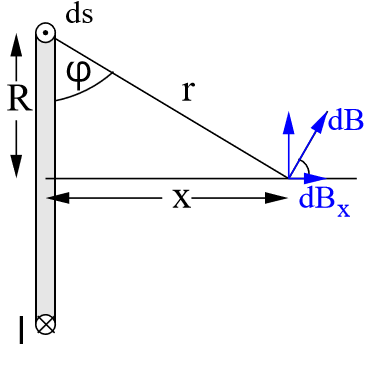
\includegraphics[width=5 cm , height=3.5 cm]{Abb1.png}
	\caption{Schematische Darstellung des Biot-Savartschen Gesetz[1].}
	\label{abb:1}
\end{figure}
Im Inneren für langgestreckten Spule (Solenoid) ist die magnetische Feldstärke $\vec{H}$
homogen und konstant während es außerhalb inhomogen ist.
Mit der Spulenlänge $l$, der Windungszahl $n$ und den Strom $I$ lässt sich das
homogene Magnetfeld mit der Formel
\begin{equation}
  B = \mu_r \mu_0 \frac{n}{l} I
  \label{eq:3}
\end{equation}
darstellen.
Eine genauere Berechnung zur Magnetfeldstärke kann folgende Form verwendet werden
\begin{equation}
  B= \frac{\mu_0 n I R^2}{2} \cdot (\frac{x-x_1}{\sqrt{(x-x_1)^2 +R^2}} - \frac{x-x_2}{\sqrt{(x-x_2)^2 +R^2}})
  \label{eq:7}
\end{equation}
Eine bildiche Veranschaulichung der Gleichung (\ref{eq:7}) steht in [2].
Wird die langgestreckte Spule zu einem Kreis gebogen so wird die Spulenanordnung
als Torus bezeichnet. Die Besonderheit des Torus ist, dass außerhalb kein Magnetfeld
existiert und im Inneren das Magnetfeld homogen ist. Somit lässt sich die Gleichung(\ref{eq:3})
mit $l= 2\pi r_T$ zu
\begin{equation}
  B = \mu_r \mu_0 \frac{n}{2\pi r_T} I
  \label{eq:4}
\end{equation}
umschreiben. Dabei ist $r_T$ der Radius des Torus.
Ein anderes Verfahren zu Herrichtung eines homogenen Magnetfeldes ist die Helmholz-Spule.
Zwei parallele Kreisspulen, die die gleiche Stromrichtung besitzen, erzeugen ein homogenes
Feld im Inneren der beiden Spulen. Eine Darstellung ist in Abbildung(\ref{abb:2}) zu sehen.
\begin{figure}[H]
  \centering
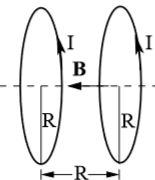
\includegraphics[width =5 cm, height = 3.5cm]{Abb2.png}
\caption{Schematische Darstellung der Helmholz-Spule[1].}
\label{abb:2}
\end{figure}
Mit Hilfe der Gleichung (\ref{eq:2}) lässt sich das Magnetfeld
\begin{equation}
  B(0)=B_1(x_1) + B_1(-x_1) = \mu_0 I \frac{R^2}{(R^2 + x^2)^{\frac{3}{2}}}
  \label{eq:5}
\end{equation}
beschreiben. Dabei ist $x=\frac{d}{2}$ mit $d$ als Abstand der beiden Spulen gemeint.\\
Ferromagnetische Materialien wie z.B. Eisen, Kobalt oder Nickel besitzen ohne ein äußeres Magnetfeld
ein permanentes magnetisches Moment. Magnetischen Momente richten sich in einzelnen Bereichen (Weißsche Bezirke)
parallel zu einander aus. Ohne äußeres Feld ist die Ausrichtung der Weißschen Bezirke statisch verteilt.
Mit einem äußeren Magnetfeld gibt es eine Richtungsänderung und zu einer Vergrößerung des Bezirks.
Dies wird solange ausgeführt bis alle magnetischen Momente mit der Ausrichtung vom Magnetfeld übereinstimmen.
Für ferromagnetische Materialien ist die relative Permeabilität $\mu_r$ sehr hoch, somit ist die Gültigkeit der
Gleichung (\ref{eq:1}) ungültig.
Die Hysteresekurve beschreibt diese Nicht-linearität und ist in Abbildung (\ref{abb:3}) dargestellt.
\begin{figure}[H]
  \centering
  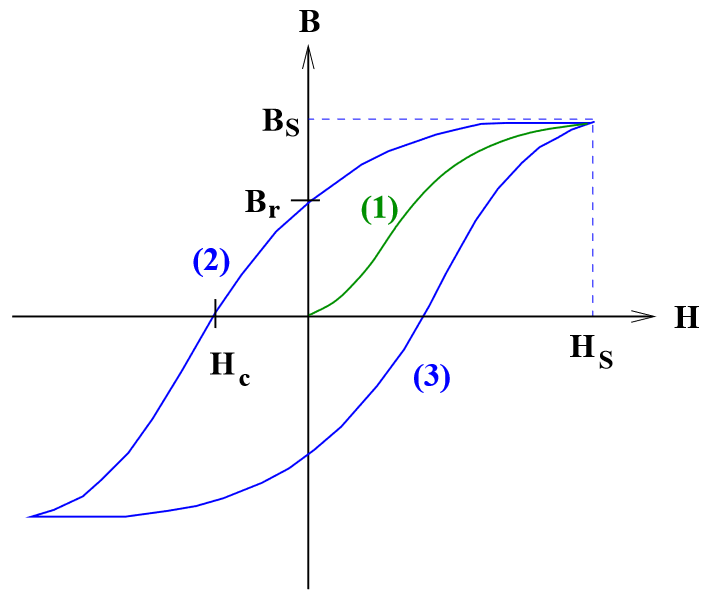
\includegraphics[width=10cm, height= 7cm]{Abb3.png}
  \caption{Schematische Darstellung einer Hysteresekurve}
  \label{abb:3}
\end{figure}
Liegt ein äußeres Magnetfeld an so wird die \textbf{1} in der Abbildung (\ref{abb:3}) eine
Neukurve dargestellt. Sie erreicht nach einiger Zeit ein Sättigungswert $B_s$. Beim Abschalten
des äußeren Magnetfeldes, bleibt noch beim Ferromagnet eine "Restmagnetisierung" die
als Remanenz bezeichnet wird. Die \textbf{2} beschreibt die Koerzitivkraft um die Remanenz auf null zu bekommen.
Durch Erhöhung des Gegenfeldes wird ebenfalls ein negativen Sättigungswert erreicht.
Die \textbf{3} zeigt den Kurvenverlauf durch Erhöhung des Magnetfeldes und sie ist symmetrisch zur Hysteresekurve.
Somit wird die relative Permeabilität $\mu_r$ eine Funktion zur Feldstärke $\vec{H}$.
Die Neukurve wird durch die differentielle Permeabilität $\mu_{diff}$ beschrieben und lautet 
\begin{equation*}
  \mu_{diff} = \frac{dB}{\mu_0 \cdot dH}
  \label{eq:6}
\end{equation*}

\section{Versuchsaufbau}
Zur Bestimmung des Trägheitsmoments I wird zunächst die
die Drillachse, siehe Abbildung 2, benötigt. Die Drillachse
die über eine Spiralfeder mit einem Rahmen verbunden.
\begin{figure}[H]
  \centering
  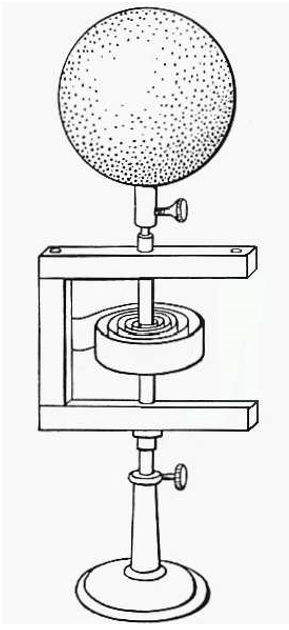
\includegraphics[width=5 cm , height= 10 cm]{Bild2.jpg}
   \caption{Schematische Darstellung des Versuchsaufbau}
\end{figure}
Auf die Achse können verschiedene Objekte angebracht werden.
%Das Eigenträgheitsmoment $I_\text{D}$ sowie die Winkelrichtgröße D lässt sich über die Schwingungsdauer T
%berechnet.

\section{Durchführung}
Zu Beginn wird die Leelaufspannung mit Hilfe eines Spannungsmessers bestimmt sowie deren Eigenwiderstand.
In Abbildung (\ref{abb:2}) werden aus unterschiedlichen Spannungsformen (in diesem Fall Gleich-,Rechteck- und Sinusspannung)
die Spannungswerte sowie Stromwerte notiert.
\begin{figure}[H]
  \centering
  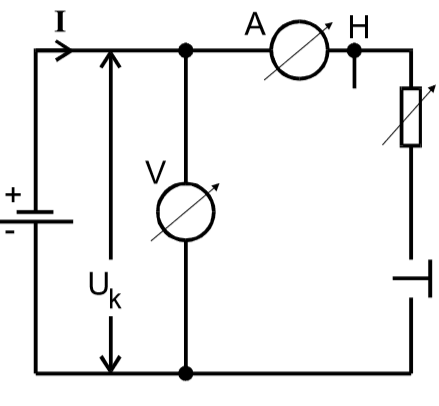
\includegraphics[width= 10 cm , height=7 cm]{Bild2.png}
  \caption{Stromkreis zu Bestimmung von $U_0$ und $R_i$ \cite{1}}
  \label{abb:2}
\end{figure}
In Abbildung (\ref{abb:3}) ist nun eine Gegenspannung angeschlossen. Dies bewirkt, dass sich der Stromfluß
ändert.
\begin{figure}[H]
  \centering
  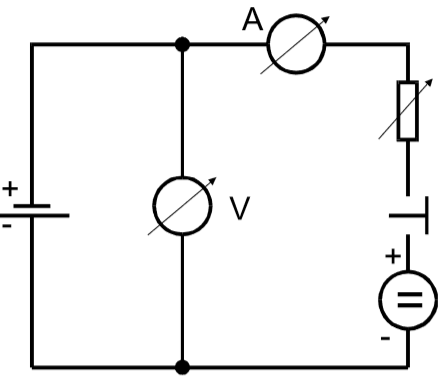
\includegraphics[width=10 cm, height= 7 cm]{Bild3.png}
  \caption{Stromkreis zu Bestimmung von $U_0$ und $R_i$ \cite{1}}
  \label{abb:3}
\end{figure}

\printbibliography{}
\nocite{*}
\end{document}
